\begin{abstract}
Neural differential distinguishers can break more rounds of block ciphers than classical single-bit methods, yet two foundational questions remain open:
where does the distinguishing signal reside in observable ciphertext data, and does this signal compose across rounds in the memoryless fashion assumed by classical differential analysis?
We answer both through a controlled study on three cipher families---\speck (ARX), \simon (Feistel), and \present (SPN)---using seven architectures under identical conditions.
Saliency and attention analysis localize the signal to XOR-difference bits, multi-bit representations outperform word-level inputs by 29\pp, and all seven architectures agree within 2\pp---confirming that the signal is intrinsic to cipher structure, not model capacity.
Transfer experiments then reveal that signal composition is family-dependent: SPN features compose hierarchically (99.1\% cross-round transfer, $p < 10^{-11}$), while ARX and Feistel features are round-specific and \emph{anti-compose}---a 5-round \speck model scores 45.5\% on 3-round data ($p < 10^{-8}$), below random chance.
VAE-based validation independently confirms that the cipher's differential propagation \emph{is} Markovian (memory/Markov MSE ratio $\approx 1.0$ across all rounds)---yet neural features still anti-compose, indicating that the networks learn round-specific representations that go beyond the Markovian differential structure.
These results fill a gap identified by a recent survey of 66~peer-reviewed papers~\citep{gerault2024sok}: no prior work jointly characterizes signal representation and compositional structure across cipher families.
\end{abstract}

\begin{figure*}[htbp]
  \centering
  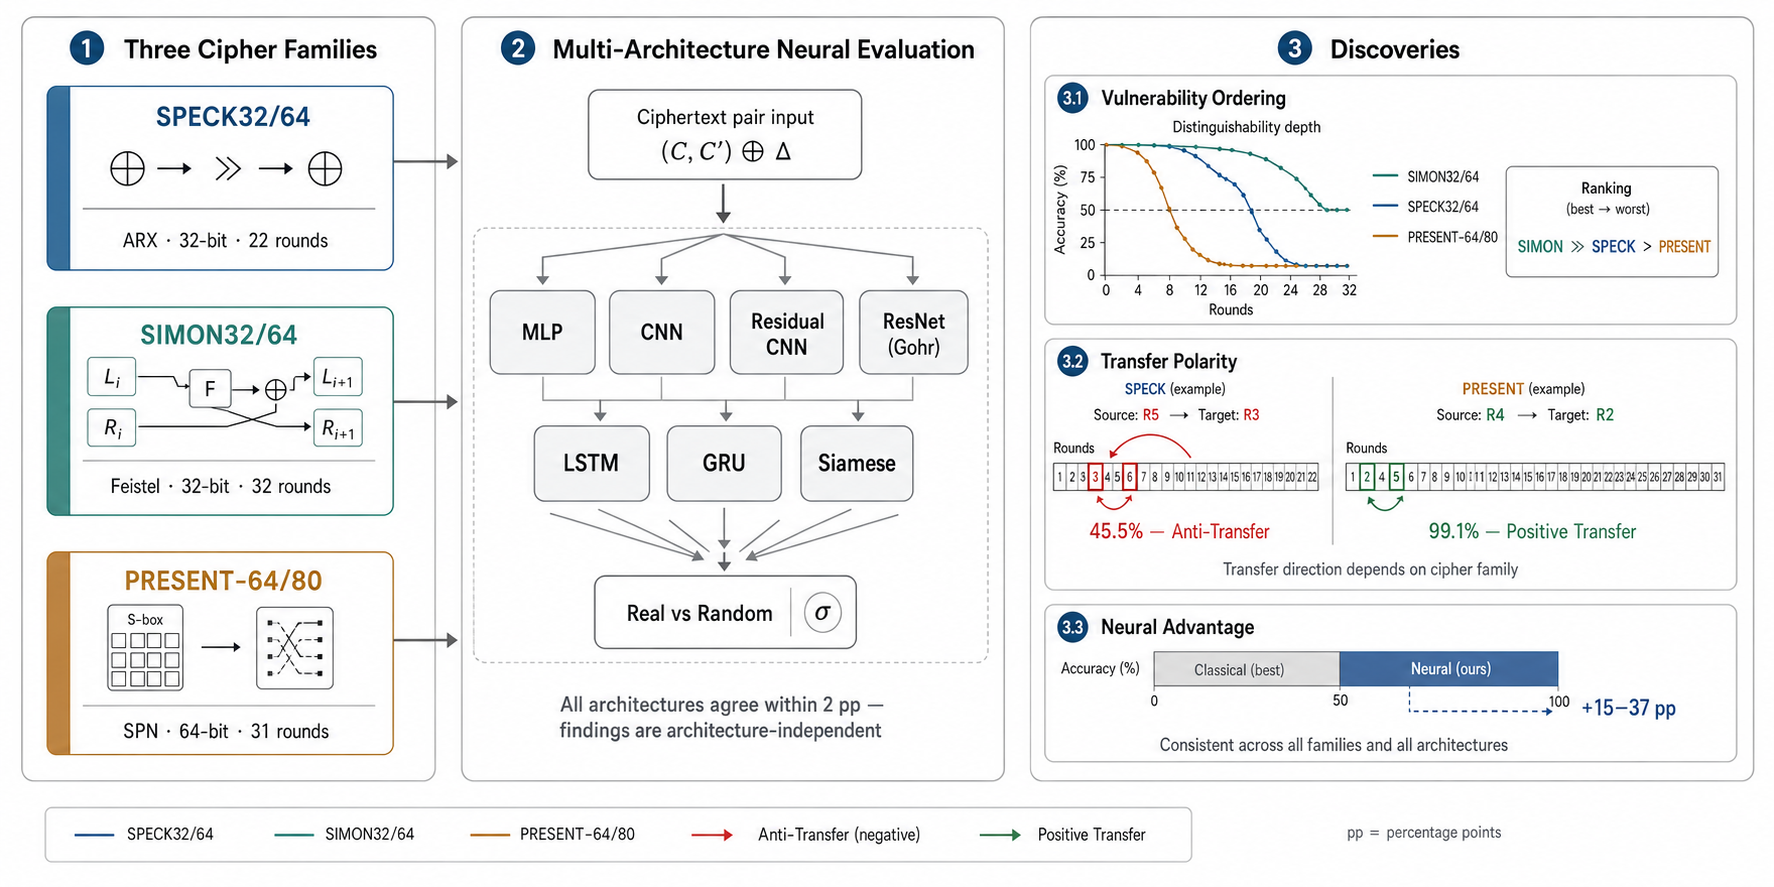
\includegraphics[width=\textwidth]{hero_fig.png}
  \caption{\textbf{Overview.}
  Identical neural distinguishers are trained on three cipher families (left) using seven architectures (center), yielding two sets of findings (right).
  \emph{Representation:} signal resides in XOR-difference bits and is architecture-independent, establishing a vulnerability ordering \simon $\gg$ \speck $>$ \present.
  \emph{Compositionality:} SPN features compose hierarchically across rounds (positive transfer $>$99\%), while ARX and Feistel features anti-compose ($<$50\%), violating the Markovian assumption that underpins classical differential cryptanalysis.}
  \label{fig:hero}
\end{figure*}
